\documentclass{easychair}

% \usepackage{doc}
\usepackage{setspace}
\usepackage{verbatim}
\usepackage{wasysym}

%----Making things more compact
\newcommand{\smalltt}[1]{\small \texttt{#1}}
\newenvironment{packed_itemize}{
\vspace*{-0.2em}
\begin{itemize}
\setlength{\partopsep}{0pt}
\setlength{\itemsep}{1pt}
\setlength{\parskip}{0pt}
\setlength{\parsep}{0pt}
}{\end{itemize}}
\newenvironment{packed_enumerate}{
\vspace*{-0.2em}
\begin{enumerate}
\setlength{\partopsep}{0pt}
\setlength{\itemsep}{1pt}
\setlength{\parskip}{0pt}
\setlength{\parsep}{0pt}
}{\end{enumerate}}
% \renewcommand{\textfraction}{0.07}
% \renewcommand{\topfraction}{0.9}
% \renewcommand{\bottomfraction}{0.9}
% \renewcommand{\floatpagefraction}{0.66}
% \setlength{\floatsep}{2.0pt plus 2.0pt minus 2.0pt}
% \setlength{\textfloatsep}{5.0pt plus 2.0pt minus 0.0pt}

\title{Stepping Stones in the TPTP World}

\author{
  Geoff Sutcliffe
}

\institute{
  University of Miami,
  Miami, USA\\
  \email{geoff@cs.miami.edu}\\
}

\authorrunning{Geoff Sutcliffe}
\titlerunning{Stepping Stones in the TPTP World}

\begin{document}
\maketitle

%--------------------------------------------------------------------------------------------------
\begin{abstract}
The first release of the TPTP problem library was made on Friday 12th November 1993. 
Since then the TPTP World (once gently referred to as the ``TPTP Jungle'') has evolved into a 
well established infrastructure that supports research, development, and deployment of ATP systems.
There have been some key developments that helped make the TPTP World a success: 
the first TPTP problem library that was first released in 1993, 
the CADE ATP System Competition (CASC) that was conceived after CADE-12 in Nancy in 1994, 
the problem difficulty ratings that were added in 1997, 
the current TPTP language that was adopted in 2003, 
the SZS ontologies that were specified in 2004, 
the TSTP solution library that was built starting around 2005, 
the Specialist Problem Classes (SPCs) used to classify problems from 2010, 
the SystemOnTPTP service that was offered from 2011, 
and 
the StarExec service that started in 2013. 
This talk reviews these stepping stones in the development of the TPTP World.
\end{abstract}
%--------------------------------------------------------------------------------------------------
\section{Introduction}
\label{Introduction}

The TPTP World \cite{Sut10,Sut17} is a well established infrastructure that supports research, 
development, and deployment of ATP systems.
Salient components of the TPTP World are
the TPTP problem library \cite{Sut09}, 
the TSTP solution library \cite{Sut10}, 
the TPTP languages \cite{SS+06}, 
the SZS ontologies \cite{Sut08-KEAPPA},
the Specialist Problem Classes (SPCs) and problem difficulty ratings \cite{SS01},
and the CADE ATP System Competition (CASC) \cite{Sut16}.
StarExec \cite{SST14} and SystemOnTPTP \cite{Sut00-CADE-17} provide computational support for
the TPTP World.
There are dependencies between these parts of the TPTP World, as shown in 
Figure~\ref{Dependencies}, forming a series of "stepping stones" from key starting points
through to happy users, who contribute to TPTP problem library.
There is another cycle of dependencies: from the TPTP problem library, to the TSTP solution 
library, to the problem difficulty ratings, and back to the TPTP problem library.
This cycle means that building these components, releases of the TPTP problem library in
particular, requires iteration until stability is reached.

\begin{figure}[htbp]
\centering
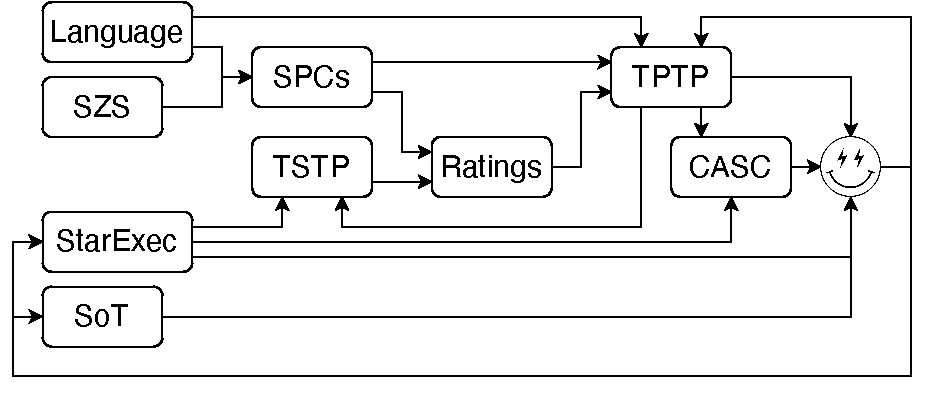
\includegraphics[width=0.75\textwidth]{Dependencies.pdf}
\caption{Dependencies between the Stepping Stones}
\label{Dependencies}
\end{figure}

Various parts of the TPTP World have been deployed in a range of applications, in both academia 
and industry.
Since the first release of the TPTP problem library in 1993, many researchers have used the 
TPTP World as an appropriate and convenient basis for ATP system research and development. 
Over the years the TPTP World has provided a platform upon which ATP users have presented their 
needs to ATP system developers, who have then adapted their ATP systems to the users’ needs.
The web page {\smalltt{\url{https://www.tptp.org}}} provides access to all components.

\paragraph{This paper is organized as follows:}

%--------------------------------------------------------------------------------------------------
\section{The TPTP Languages}
\label{Languages}

The TPTP language \cite{Sut23-IGPL} is one of the keys to the success of the TPTP World.
The language is used for writing both problems and solutions,
which enables convenient communication between systems. 
% It also enables tool exchange, tool integration, and comparable experimental results.
Originally the TPTP World supported only first-order clause normal form (CNF)
\cite{SS98-JAR}.
Over the years full first-order form (FOF)
\cite{Sut09}, 
typed first-order form (TFF)
\cite{SS+12,BP13-TFF1}, 
typed extended first-order form (TXF)
\cite{SK18}, 
typed higher-order form (THF)
\cite{SB10,KSR16}, 
and non-classical forms (NTF) \cite{SF+22} have been added.
A general principle of the TPTP language is ``we provide the syntax, you provide the semantics''.
As such, there is no a priori commitment to any semantics for the languages, although in almost 
all cases the intended logic and semantics are well known.

The formulae of problems solutions are built from {\em annotated formulae}, 
which have the form~\ldots \\
\hspace*{0.5cm}{\em language}{\tt (}{\em name}{\tt ,}
{\em role}{\tt ,}
{\em formula}{\tt ,}
{\em source}{\tt ,}
{\em useful\_info}{\tt )}\\
The {\em language}s supported are {\smalltt{cnf}} (clause normal form), {\smalltt{fof}}
(first-order form), {\smalltt{tff}} (typed first-order form), and {\smalltt{thf}}
(typed higher-order form).
The {\em role}, e.g., {\smalltt{axiom}}, {\smalltt{lemma}}, {\smalltt{conjecture}}, defines the 
use of the formula in an ATP system.
In a {\em formula}, terms and atoms follow Prolog conventions -- functions and predicates start 
with a lowercase letter or are {\tt '}single quoted{\tt '}, and variables start with an uppercase 
letter.
The language also supports interpreted symbols, which either start with a {\tt \$}, e.g., the 
truth constants {\smalltt{\$true}} and {\smalltt{\$false}}, or are composed of 
non-alphabetic characters, e.g., integer/rational/real numbers such as 27, 43/92, -99.66.
The logical connectives in the TPTP language are
{\tt !}, {\tt ?}, {\tt {\raisebox{0.4ex}{\texttildelow}}}, {\tt |}, {\tt \&}, {\tt =>}, {\tt <=},
{\tt <=>}, and {\tt <{\raisebox{0.4ex}{\texttildelow}}>},
for the mathematical connectives
$\forall$, $\exists$, $\neg$, $\vee$, $\wedge$, $\Rightarrow$, $\Leftarrow$, $\Leftrightarrow$, 
and $\oplus$ respectively.
Equality and inequality are expressed as the infix operators {\tt =} and {\tt !=}.
The {\em source} and {\em useful\_info} are optional.
Figure~\ref{ExampleFormula} shows an example with typed higher-order formulae.

\begin{figure}[htb]
{\footnotesize
{\setlength{\baselineskip}{3mm}
\begin{verbatim}
%------------------------------------------------------------------------------
thf(beverage_decl,type,   beverage: $tType ).
thf(syrup_decl,type,      syrup: $tType ).
thf(coffee_type,type,     coffee: beverage ).
thf(mix_type,type,        mix: beverage > syrup > beverage ).
thf(heat_type,type,       heat: beverage > beverage ).
thf(heated_mix_type,type, heated_mix: beverage > syrup > beverage ).
thf(hot_type,type,        hot: beverage > $o ).

thf(heated_mix,axiom,
    ( heated_mix
    = ( ^ [B: beverage,S: syrup] : ( heat @ ( mix @ B @ S ) ) ) ) ).

thf(hot_mixture,axiom,
    ! [B: beverage,S: syrup] : ( hot @ ( heated_mix @ B @ S ) ) ).

thf(heated_coffee_mix,axiom,
    ! [S: syrup] : ( ( heated_mix @ coffee @ S ) = coffee ) ).

thf(hot_coffee,conjecture,
    ? [Mixture: syrup > beverage] :
      ~ ? [S: syrup] :
          ( ( ( Mixture @ S ) = coffee )
          & ( hot @ ( Mixture @ S ) ) ) ).
%------------------------------------------------------------------------------
\end{verbatim}
}}
\caption{THF annotated formulae}
\label{ExampleFormula}
\end{figure}

%--------------------------------------------------------------------------------------------------
\section{The TPTP Problem Library}
\label{TPTP}

The development of the TPTP World started with the TPTP problem library in mid-1992, as a 
collaboration between Geoff Sutcliffe at the University of Western Australia (James Cook 
University from 1993), and Christian Suttner at the Technische Universit{\"a}t M{\"u}nchen.
The TPTP problem library is managed in the manner of a software product, in the sense that fixed 
releases are made.
Each release is identified by a release number in the form v$Version$.$Edition$.$Patch$:
the $Version$ enumerates major new releases of the TPTP in which important new features have 
been added,
the $Edition$ is incremented each time new problems are added to the current version, and
The $Patch$ level is incremented each time errors, found in the current edition, are corrected. 
The first public release, TPTP v1.0.0, was made on 12th November 1993.

The problems in the TPTP are classified into {\em domains} that reflect the natural hierarchy of 
scientific domains.
Seven main fields are defined: logic, mathematics, computer science, science \& engineering, 
social sciences, arts \& humanities, and other. 
Each field is subdivided into domains, each identified by a three-letter mnemonic, e.g., the
social science field has three domains: Social Choice Theory (SCT), Management (NGT), and
Geography (GEG).

Table~\ref{tab:Releases} lists the versions of the TPTP up to v9.0.0, with the new feature added, 
the number of problem domains, and the number of problems.\footnote{%
The data for v9.0.0 is an estimate, because this paper was written before the release was
finalised.}
The number of domains indicates the semantic diversity of the TPTP problems, while the number
of problems indicates the size of the TPTP problem library.
The attentive reader might note that many releases have been made in July/August.
This is because the CADE ATP System Competition (CASC - see Section~\ref{CASC}), has an 
influence on the release cycle of the TPTP. 

\begin{table}[htb]
\begin{center}
\setlength{\tabcolsep}{4pt}
\begin{tabular}{ll|l|rr}
Release & Date     & Changes                                              & Domains & Problems \\
\hline
v1.0.0  & 12/11/93 & First public release, only CNF \cite{SS98-JAR}       &      23 &     2295 \\
v2.0.0  & 05/06/97 & FOF \cite{Sut09} and ratings (Section~\ref{Ratings}) &      28 &     3277 \\
v3.0.0  & 11/11/04 & New TPTP language \cite{SS+06}                       &      32 &     7267 \\
v4.0.0  & 04/07/09 & TH0 (monomorphic typed higher-order) \cite{SB10}     &      41 &    16512 \\
v5.0.0  & 16/09/10 & TF0 (monomorphic typed first-order) \cite{SS+12}     &      45 &    18480 \\
v6.0.0  & 21/09/13 & TF1 (polymophic typed first-order) \cite{BP13-TFF1}  &      48 &    20306 \\
v7.0.0  & 24/07/17 & TH1 (polymophic typed higher-order) \cite{KSR16}     &      53 &    21851 \\
v8.0.0  & 19/04/22 & TXF (typed extended first-order) \cite{SK18}         &      54 &    24785 \\
v9.0.0  & ??/07/24 & NTF (non-classical typed first-order) \cite{SF+22}   &      55 &    25598 \\
\end{tabular}
\end{center}
\caption{Overview of TPTP releases}
\label{tab:Releases}
\end{table}

TPTP problem files present the logical formulae in a format that is both human and machine 
readable, and additionally provide useful information for users.
The file names are built from the domain acronym, a 3 digit problem number, a separator that
indicates the syntax ({\tt -} for CNF, {\tt +} for FOF, {\tt \_} for TFF, {\tt \verb|^|} for THF),
optional digits for the problem size, and a problem version number.
Each file has three sections: a header, optional includes, and the formulae.

The header section contains information for users, formatted as comments in four parts:
the first part identifies and describes the problem;
the second part provides information about occurrences of the problem
in the literature and elsewhere;
the third part provides semantic and syntactic characteristics of the problem;
the last part contains comments and bugfix information.
The include section is optional, and if used contains {\tt include} directives for axiom files,
which in turn have the same three-part format as problem files.
Their inclusion avoids the need for duplication of the formulae in commonly used axiomatizations.
The formula section contains annotated formulae, as described in Section~\ref{Languages}.
Figure~\ref{ExampleHeader} shows an example header and {\tt include} section.
The header fields are self-explanatory, but of particular interest are the {\tt Status} field 
that is explained in Section~\ref{SZS}, the {\tt Rating} field that is explained in 
Section~\ref{Ratings}, and the {\tt SPC} field that is explained in Section~\ref{SPCs}.

\begin{figure}[htb]
{\footnotesize
{\setlength{\baselineskip}{3mm}
\begin{verbatim}
%------------------------------------------------------------------------------
% File     : DAT016_1 : TPTP v8.2.0. Bugfixed v5.1.0.
% Domain   : Data Structures
% Problem  : Some element is 53
% Version  : [PW06] axioms.
% English  : Show that some element of the array has the value 53.

% Refs     : [PW06]  Prevosto & Waldmann (2006), SPASS+T
%          : [Wal10] Waldmann (2010), Email to Geoff Sutcliffe
% Source   : [Wal10]
% Names    : (40) [PW06]

% Status   : Theorem
% Rating   : 0.25 v8.2.0, 0.12 v7.5.0, 0.30 v7.4.0, 0.12 v7.3.0, etc.
% Syntax   : Number of formulae    :    6 (   1 unt;   3 typ;   0 def)
%            Number of atoms       :   12 (   5 equ)
%            Maximal formula atoms :    4 (   2 avg)
%            Number of connectives :    4 (   0   ~;   1   |;   1   &)
%                                         (   0 <=>;   2  =>;   0  <=;   0 <~>)
%            Maximal formula depth :    6 (   5 avg)
%            Maximal term depth    :    3 (   1 avg)
%            Number of FOOLs       :    5 (   5 fml;   0 var)
%            Number arithmetic     :   16 (   2 atm;   2 fun;   5 num;   7 var)
%            Number of types       :    2 (   1 usr;   1 ari)
%            Number of type conns  :    5 (   2   >;   3   *;   0   +;   0  <<)
%            Number of predicates  :    3 (   1 usr;   0 prp; 2-2 aty)
%            Number of functors    :    9 (   2 usr;   5 con; 0-3 aty)
%            Number of variables   :   10 (   9   !;   1   ?;  10   :)
% SPC      : TF0_THM_EQU_ARI

% Comments : The array contains integers.
% Bugfixes : v5.1.0 - Fixed conjecture
%------------------------------------------------------------------------------
%----Includes axioms for arrays
include('Axioms/DAT001_0.ax').
%------------------------------------------------------------------------------
\end{verbatim}
}}
\caption{Header of problem {\tt DAT016\_1}.}
\label{ExampleHeader}
\end{figure}


This section has naturally focused on the successful parts of the TPTP history.
There have also been some failed developments and suboptimal (in retrospect) decisions \frownie{}.
For example, in 2015 there was an attempt to develop a description logic form for the TPTP 
language. 
While some initial progress was made, it ground to a halt without support from the description 
logic community.
A suboptimal design decision, rooted in the early days of the TPTP, is the naming scheme used for 
problem files. 
The naming scheme uses three digits to number the problems in each domain, thus setting a limit 
of 1000 problems, which failed to anticipate the numbers of problems that would be contributed 
to some of the problem domains.
This has been overcome by creating multiple domain directories where necessary, but if it were 
to be done again, six or eight digit problem numbers shared across all domains would be an 
improvement.

%--------------------------------------------------------------------------------------------------
\section{The TSTP Solution Library}
\label{TSTP}

%--------------------------------------------------------------------------------------------------
\section{The SZS Ontologies}
\label{SZS}

%--------------------------------------------------------------------------------------------------
\section{Specialist Problem Classes}
\label{SPCs}

%--------------------------------------------------------------------------------------------------
\section{Problem Difficulty Ratings}
\label{Ratings}

%--------------------------------------------------------------------------------------------------
\section{StarExec and SystemOnTPTP}
\label{StarExec}

%--------------------------------------------------------------------------------------------------
\section{The CADE ATP System Competition}
\label{CASC}

%--------------------------------------------------------------------------------------------------
\section{TPTP World Users}
\label{Users}

%--------------------------------------------------------------------------------------------------
\section{Conclusion}
\label{Conclusion}

This paper 

Currently this work is being extended to 

%--------------------------------------------------------------------------------------------------
\bibliographystyle{plain}
\bibliography{Bibliography.bib}
%--------------------------------------------------------------------------------------------------
\end{document}
%--------------------------------------------------------------------------------------------------
